\documentclass[twocolumn]{article}

% Feel free to add more packages
\usepackage{float, amsmath, amssymb, mathtools}
\usepackage{graphicx, caption, color}
\usepackage{tabularx, fullpage}
%\usepackage{kotex}
%\usepackage{multicol}
\setlength{\columnsep}{1cm}
\usepackage{comment, cite, wrapfig}
\usepackage[utf8]{inputenc}
\usepackage[hidelinks]{hyperref}
%\usepackage{geometry}
\hypersetup{breaklinks=true}
\urlstyle{same}

\newcommand{\red}[1]{{\bf \color{red}#1}}
\newcommand{\blue}[1]{{\bf \color{blue}#1}}
\newcommand{\cut}[1]{}


\begin{document}

\title{Natural Language Interface for Relational Database\\
	\small{Midterm Report}}

%Authors in alphabetical order of last names
\author{Yilin Gao \\
	\small \texttt{yilin.gao@duke.edu} \and 
	Keping Wang \\
	\small \texttt{kw238@duke.edu} \and 
	Chengkang Xu \\
	\small \texttt{cx33@duke.edu} }
	
\date{\today}
\maketitle

%%%================================================================%%%
\section{Introduction}\label{sec:introduction}

This project is going to build a natural language interface for relational databases, following the ideas of Li et al. (2014)\cite{li2014}. Constructing an Interactive Natural Language Interface for Relational Databases. Here we only focus on how to select data (no insert, add, drop).
	
This project is of course meaningful. Since SQL queries are not easy for everyone to learn, this interface will be an excellent tool for everyone to query data from relational databases. For example, users of a searching engine are very likely type in a question like "Which river is the longest river in the world?", and the searching engine should transform this question into SQL queries and execute it against its huge database. If the searching engine is not able to understand the meaning of the question correctly, it will fail to provide users with correct answer.
    
People have been working on this for decades, but it is really more about the understanding of natural language rather than the generating of SQL queries. Because SQL queries have well defined grammars and all the tricky ambiguities lie in natural languages. Thankfully, nowadays we have high accuracy dependency syntax parser to make NLIDB really feasible. In this course project, we are both interested in natural language processing and its application in database application.
    
In the past, many natural language interfaces to databases (NLIDBs) has been built to better translate natural language into database queries. NLIDBs have many advantages over other widely used accepted query interfaces, but they have not been adopted widely. This is because understanding natural language is hard. It is important for NLIDBs to improve its parsing and transformation systems, and interact with users more effectively. \cite{li2014}
      
      We intend to closely follow the paper \cite{li2014}. The main steps of translating a natural language to an SQL query are as follows:

\begin{enumerate}
      \item Parse the natural language using a dependency parser (Stanford NLP Parser).
      \item Map the parse tree nodes to SQL keywords and table and attribute names.
      \item Adjust the structure of the parse tree to make it follow the structure of an SQL query. The result of this procedure is then called a query tree.
      \item Translate the query tree to an SQL query.
      \item During step 2 and 3 there is interactive communication with the user to let the user choose the desired mappings or structures out of ranked choices.
\end{enumerate}
        
Steps 2 - 4 are the most complicated parts, because we need to code up the grammatical rules that the parse trees should follow to get translated to SQL queries, which requires deep understanding of the SQL language. \textbf{Each member of our group will focus on one step among steps 2 - 4.} Also there will be a user interface in our system coded with Java.

We plan to use \textit{Microsoft Academic Search Database} for testing as in \textit{Fei Li 2014}, but PostgreSQL as our database (since we've learned to use it in CS516).
	
Possible obstacles we might encounter are:
\begin{itemize}
\item The system is really complicated, and except for the available Standford NLP Parser, we need to code the user interface, parser tree node mapper, parser tree structure adjuster and the query tree translator by ourselves.
\item We are not very familiar with NLP, and have no experience in translating natural language into SQL language, so we should study related knowledge by ourselves.
\end{itemize}

%%%================================================================%%%
\section{Related Work}
NLIDBs which we will study belongs to QA systems. Modern QA systems have developed into many categories, like natural language, visual questions, and AI ability test. Here we focus on the development of natural language QA systems. These systems can develop on structured data like databases and semi-structured or unstructured data like web information. \cite{QATutorial}
      
Early work in natural language database systems is usually based on small scale database. These databases are of simple schema and small numbers of entities, thus can only answer a small set of questions. Moreover, their natural language parsing systems can only support ad-hoc methods and semantic parsing. In other words, early work will produce ambiguity if database is scalable and natural language queries are "open-domain". And without the help of machine learning methods, early QA systems cannot update their parsing methods as they accumulate more data.
      
As research goes deeper, natural language database systems can support larger databases and more complicated query formats. The mainstream approach is semantic parsing of questions. It can map natural language questions to logic forms or structured queries, and produce accurate answers when the query is complete and clear. And there exist several challenges in this method. The accuracy of answering questions will decline if the input language is ambiguous, if the logic relationship of the query is complicated, or if the database is very large. In recent years, a huge amount of literature has developed many innovative methods to reduce ambiguity during interpretation of natural language, transformation from natural language into SQL queries, and searching into database. These attempts have achieved satisfactory improvements in output accuracy. But ambiguity due to complexity in query languages and datasets is still the major challenge in this field, and researchers are still working on new methods to improve QA systems' performance.
      
Our problem differs from previous literature in that, we mainly focus on how to transform parsed natural language into query trees and SQL queries, and we will use a third-party package to finish parsing tasks. But at present, research focuses on how to increase parsing accuracy with cutting-edge methods in machine learning, and how to increase accuracy when the query structure is complicated and the dataset is huge. This is because our major purpose is to get hands-on experience in how to establish such a large system and how the system operates. We can focus on improving system efficiency in future work.


%%%================================================================%%%
\section{Problem Definition}
NLIDBS - Natural Language Interfaces to Databases, a computer human interface that is capable of understanding varieties of ambiguous input and executing corresponding actions on database.
      
Parse tree structure adjustor - It is used to adjust the sequence of the SQL keywords that are parsed from mapper to correctly understand and execute the intended query.  Once the natural language keywords have been matched with SQL keywords, it will inserted some keywords if missing to better interpret the input and  generate valid SQL query.
      
Parse tree node mapper - This is a mapper that maps keywords in natural language to SQL keywords. The mapper will try to output the most accurate match between natural language keyword and SQL keyword. If no match is found, it will ignore the word. Our current strategy is to mapping keywords based on its neighbour words (i.e. if two words are adjacent, they are considered as relevant and it will affect the interpret of words that have multiple interpretations).
      
Dependency parser - Dependencies that is used to parse natural language query linguistically.  We will be using Stanford Parser to perform the task.
      
NV node - Every node in the parse tree, which has one or more candidate map is an NV node.
	
In Fei Li’s research, he states several methods that he used in building the NLIDBS. First of all, he defined different types of nodes. Every node type has a specified pool of corresponding natural language words. With the definition of these types, keywords in natural language can be organized more accurately. Second, he proposed that in order for mapping to work more accurately, database schema should be meaningful and human-legible. When similar meaning words present, they will be more likely to be matched with corresponding SQL keywords correctly. Third, after all keywords have been translated into SQL keywords, there will be more than one candidate maps returned for user to choose. Once user chooses the one that fits user’s intended query the best, the candidate map is finalized. Li’s paper proposed procedures for handling and parsing natural language into SQL.\cite{li2014} Follow the idea, we will implement our own algorithm for solving similar problems.

Currently, there is not many easy-to-use NLIDBS available. Our goal is to create an interface that allows user to input natural language and process it into SQL. Users can type in query in natural language in the text box. Parser will validate the input and execute corresponding query.


%%%================================================================%%%
\section{Algorithms}
Our first step in implementing the translation process is to parse the natural language into SQL keywords using a predefined mapping. Our mapping is written in NodeMapper.java. Since we are still testing the parse, the mapping only limits to a few keywords, such as: return, equals, all, etc. If there is no exact match in our predefined maps, the mapping will try to match word with the column name based on similarity. The similarity composes of two parts. First part is lexical similarity, which is the similarity of the appearance of characters. We are using Jaccord coefficient to compute the lexical similarity. Second part is semantic similarity. We are using libraries from wordNet to compute it. After we have both similarity, we use the higher one in these two as the similarity score between word and column name. In case, the words is meaningless, we also add a meaningless option after the computation of similarity is finished. User will need to choose the most similar option from the list generated from similarity computation. 


%%%================================================================%%%
\section{System Design}

\begin{figure*}[ht]
  \centerline{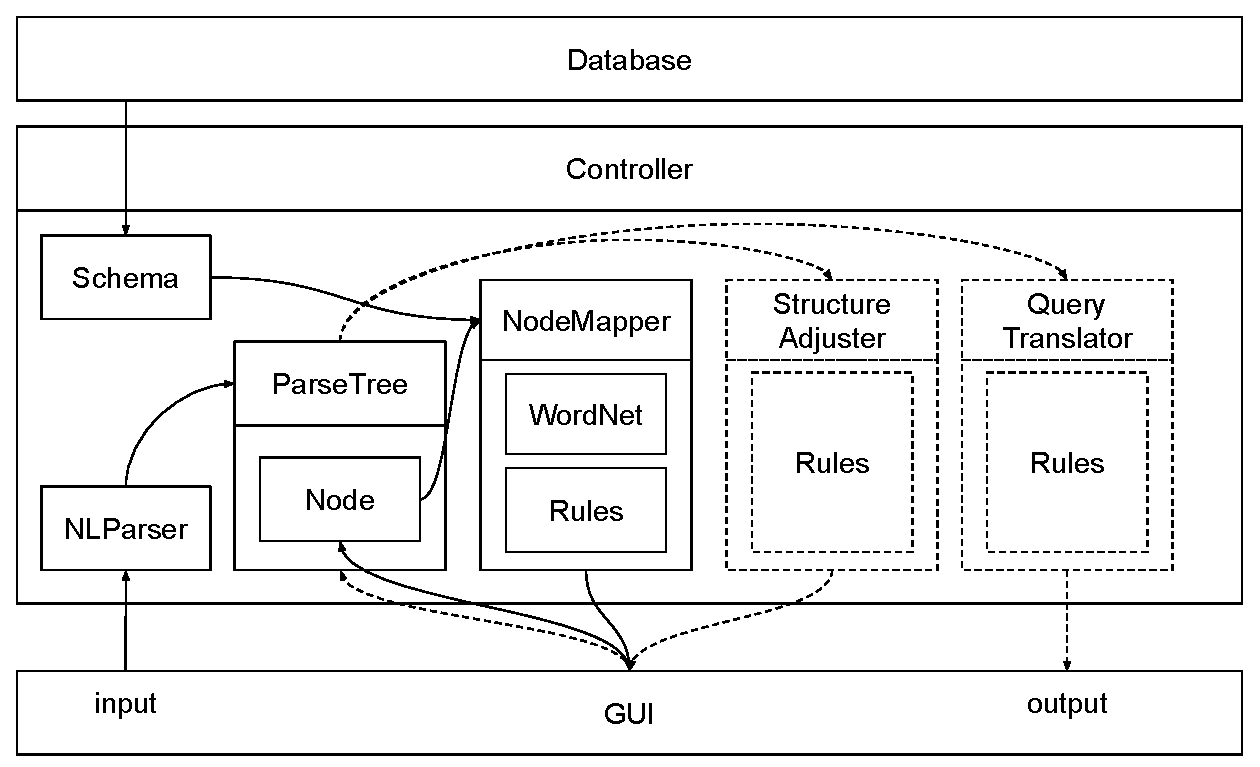
\includegraphics[width=0.8\linewidth]{figures/nlidb_system_diagram.pdf}}
  \caption{System Diagram}
\end{figure*}

Our current system is implemented in java, using maven as the project management tool. The source code are divided into three parts: model, view, and control. The controller here wraps many models as attribute variables, and it takes charge of the interaction between database and the view (GUI). We use JavaFX for the GUI.

Figure 1 is a diagram of our system. The boxes with solid frame lines are the ones we've already written, and the boxes with dashed frame lines are to be completed in the future.

Below we’ll introduce the two steps that we’ve completed: parsing natural language into a parse tree, and mapping the nodes of the parse tree to SQL components.

\subsection{Natural Language Parser}
We write the NLParser class to parse natural language from the user input in GUI to a dependency parse tree. The NLParser is just a wrapper of the Standford NLP pos-tagger and dependency syntax parser. A natural language sentence is first tagged with part-of-speech labels, and then parsed with dependency parser to a ParseTree.

A ParseTree consists of an array of Nodes. Each Node has information about the natural language word and its corresponding SQL component. A Node also contains parent and children links pointing to other Nodes in the ParseTree.

\subsection{Node Mapper}
Then we map each of the Node into an SQL component. We iterate over the tree and map each Node according to a certain Node Type in Figure 2, according to predefined rules. There are 7 node types in total, and 5 of them, SN, ON, FN, QN, and LN have hard-coded mapping rules. For example, map word “return” or “Return” to an “SN” node with value “SELECT”. A word will first be searched against these five Node Types. If there is no match, the search will go on to the remaining two types, NN and VN.

\begin{figure}[ht]
  \centerline{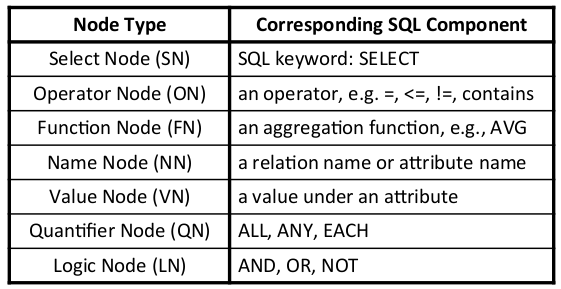
\includegraphics[width=0.9\linewidth]{figures/nodes_mapping_rules.png}}
  \caption[caption for nodes mapping rules]{Nodes Mapping Rules\protect\footnotemark}
\end{figure}
\footnotetext{Taken from \cite{li2014}.}

The remaining two types, Name Node and Value Node, are decided by searching over the database for matching names or values. The matching of word to names or values are decided by the word similarity score of two words.The word similarity score here is the maximum of semantic similarity and lexical similarity.

Semantic similarity is the WUP similarity function using WordNet. WordNet is a net of synonym sets (synsets) connected with semantic and lexical pointers. Two most important semantic pointers are hypernym and hyponym, which connect the synsets to the tree that we are interested here, as Figure 3. In Figure 3, the WUP similarity between $C1$ and $C2$ is:

$$ Sim_{WUP} = \frac{2*N3}{N1+N2+2*N3} $$

\begin{figure}[ht]
  \centering
  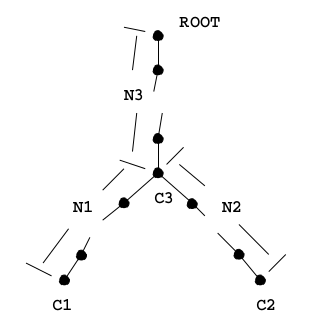
\includegraphics[width=0.7\linewidth]{figures/wordnet_tree.png}
  \caption[caption for wordnet tree]{WUP word similarity.\protect\footnotemark }
\end{figure}
\footnotetext{Taken from \cite{wu1994verbs}.}

One thing to note about WordNet is that each word can be in multiple synsets, and each synset can have multiple parents, so we use breadth-first-seach to find the lowest of all possible common parents of two words.

For lexical similarity between two words, we use the Jaccard coefficient:

$$ J(A, B) = \frac{|A \cap B|}{|A \cup B|}$$

where $A$ and $B$ are the set of characters of the two words respectively. The Jaccard coefficient may not be as good for measuring the lexical similarity of two words (as edit distance), but it is currently still used because it is a measrure in range (0,1), which makes it easily compared with the WUP semantic similarity.

To search over the database, we first visit the database, retrieve its schema, and store the Schema Graph as an attribute variable in the Controller class, so that each node mapping task don’t have to go through the slow database query. The Schema contains the table names, the column names of each column, and some sample distinct values of each column, such that they can be searched over to map Name Node or Value Node.

Once we have the word similarity scores of one word to names and values in database, we rank different mapping choices by their similarity score, and return the highest several choices to the GUI for the user to choose. Here we add another node type for the user to choose from, that is “UNKNOWN”, which means that node doesn’t correspond to any meaningful SQL component. These meaningless nodes will be removed in later steps.

Figure 4 is an example of a parse tree with nodes mapped to SQL components. The left part is a parse tree, and the right part is the mappings of all its nodes.

\begin{figure}[ht]
  \centerline{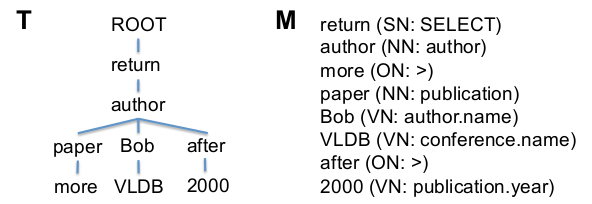
\includegraphics[width=0.9\linewidth]{figures/nodes_mapping_example.png}}
  \caption[caption for nodes mapping example]{Node Mapping Example.\protect\footnotemark }
\end{figure}
\footnotetext{Taken from \cite{li2014}.}



%%%================================================================%%%
\section{Experiments}

\begin{figure*}[ht]
  \centerline{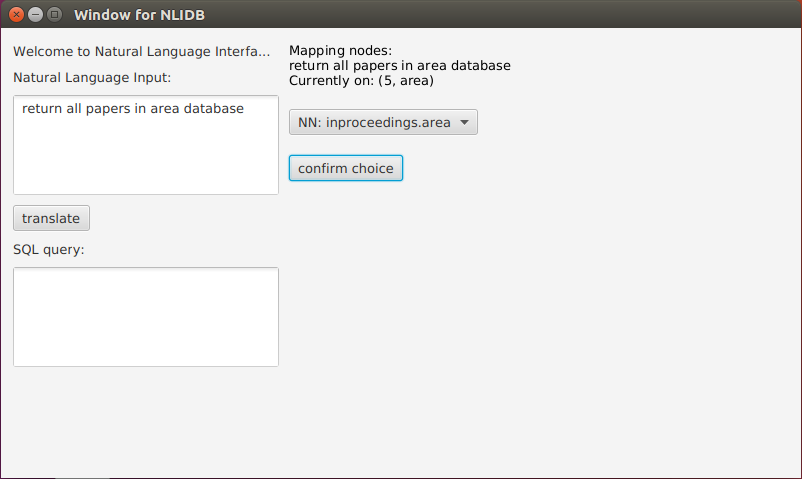
\includegraphics[width=0.7\linewidth]{figures/gui_nodes_mapping.png}}
  \caption{GUI during Node Mapping}
\end{figure*}

The JavaFX application runs on JVM, and we’ve tested it on an Ubuntu 16.04 machine. We are using JDBC to connect to the PostgreSQL database of dblp, which we used in homework 1.

Figure 5 is a screenshot of our application during the nodes mapping stage. The upper left part is where the user input comes. The bottom left part is supposed to be the translated SQL query (which hasn’t been completed). The upper left part shows the current information on nodes mapping. The choice box showing “NN: inproceedings.title” contains a drop down list of node types and values for the user to choose from. Once the user confirms the choice by pressing the “confirm choice” button, the app will go on to map the next word. The mapping choices will only be shown to the user if the word doesn’t match with the five predefined node types.

Currently we’ve only defined very limited number of explicit rules for nodes mapping. We plan to tune the app after we’ve completed writing the whole process of translation. The nodes mapping for name nodes and value nodes doesn’t work perfectly well, maybe in the future we will try some more sensible measures of word similarity. But it is ok for now, since the users can almost always find the right name node or value node from the multiple choices.

%%%================================================================%%%
\section{Contributions of Project Members}

\begin{enumerate}
\item {\bf Author-1}
\begin{itemize}
\item {\bf Midterm:}
\item {\bf Final:}
\end{itemize}
\item {\bf Author-2}
\begin{itemize}
\item {\bf Midterm:}
\item {\bf Final:}
\end{itemize}
\item {\bf Author-3}
\begin{itemize}
\item {\bf Midterm:}
\item {\bf Final:}
\end{itemize}
\end{enumerate}

\Urlmuskip=0mu plus 1mu\relax
\bibliographystyle{abbrv}
\bibliography{nlidb}

\end{document}